\documentclass[10pt,a4paperpaper,]{article}
\usepackage{lmodern}
\usepackage{amssymb,amsmath}
\usepackage{ifxetex,ifluatex}
\usepackage{fixltx2e} % provides \textsubscript
\ifnum 0\ifxetex 1\fi\ifluatex 1\fi=0 % if pdftex
  \usepackage[T1]{fontenc}
  \usepackage[utf8]{inputenc}
\else % if luatex or xelatex
  \ifxetex
    \usepackage{mathspec}
  \else
    \usepackage{fontspec}
  \fi
  \defaultfontfeatures{Ligatures=TeX,Scale=MatchLowercase}
\fi
% use upquote if available, for straight quotes in verbatim environments
\IfFileExists{upquote.sty}{\usepackage{upquote}}{}
% use microtype if available
\IfFileExists{microtype.sty}{%
\usepackage{microtype}
\UseMicrotypeSet[protrusion]{basicmath} % disable protrusion for tt fonts
}{}
\usepackage[margin=1in]{geometry}
\usepackage{hyperref}
\hypersetup{unicode=true,
            pdfborder={0 0 0},
            breaklinks=true}
\urlstyle{same}  % don't use monospace font for urls
\usepackage{longtable,booktabs}
\IfFileExists{parskip.sty}{%
\usepackage{parskip}
}{% else
\setlength{\parindent}{0pt}
\setlength{\parskip}{6pt plus 2pt minus 1pt}
}
\setlength{\emergencystretch}{3em}  % prevent overfull lines
\providecommand{\tightlist}{%
  \setlength{\itemsep}{0pt}\setlength{\parskip}{0pt}}
\setcounter{secnumdepth}{0}
% Redefines (sub)paragraphs to behave more like sections
\ifx\paragraph\undefined\else
\let\oldparagraph\paragraph
\renewcommand{\paragraph}[1]{\oldparagraph{#1}\mbox{}}
\fi
\ifx\subparagraph\undefined\else
\let\oldsubparagraph\subparagraph
\renewcommand{\subparagraph}[1]{\oldsubparagraph{#1}\mbox{}}
\fi

\date{}

\begin{document}

\section{List of useful functions}\label{list-of-useful-functions}

There are four libraries imported for this analysis:
\texttt{matplotlib}, \texttt{numpy}, \texttt{pandas}.

\begin{itemize}
\tightlist
\item
  \texttt{numpy} is used for performing mathematical operations on
  arrays
\item
  \texttt{matplotlib} allows graphs to be plotted
\item
  \texttt{pandas} provides an interface for manipulating datasets
\end{itemize}

The list below gives some functions that you will find useful, although
you can use other functions from the libraries given. Clicking on the
heading of each function will take you to the function's main
documentation page.

\subsection{numpy}\label{numpy}

\begin{longtable}[]{@{}ll@{}}
\caption{\href{http://docs.scipy.org/doc/numpy/reference/generated/numpy.sqrt.html}{\texttt{numpy.sqrt(n)}}}\tabularnewline
\toprule
\begin{minipage}[b]{0.47\columnwidth}\raggedright\strut
Description\strut
\end{minipage} & \begin{minipage}[b]{0.47\columnwidth}\raggedright\strut
Example\strut
\end{minipage}\tabularnewline
\midrule
\endfirsthead
\toprule
\begin{minipage}[b]{0.47\columnwidth}\raggedright\strut
Description\strut
\end{minipage} & \begin{minipage}[b]{0.47\columnwidth}\raggedright\strut
Example\strut
\end{minipage}\tabularnewline
\midrule
\endhead
\begin{minipage}[t]{0.47\columnwidth}\raggedright\strut
Return the square root of \texttt{n}\strut
\end{minipage} & \begin{minipage}[t]{0.47\columnwidth}\raggedright\strut
\texttt{\textgreater{}\ a\ =\ numpy.array({[}1,\ 4,\ 9{]})}

\texttt{\textgreater{}\ numpy.sqrt(a)}

\texttt{numpy.array({[}1,\ 2,\ 3{]})}\strut
\end{minipage}\tabularnewline
\bottomrule
\end{longtable}

\begin{longtable}[]{@{}ll@{}}
\caption{\href{http://docs.scipy.org/doc/numpy/reference/generated/numpy.mean.html}{\texttt{numpy.mean(data)}}}\tabularnewline
\toprule
\begin{minipage}[b]{0.47\columnwidth}\raggedright\strut
Description\strut
\end{minipage} & \begin{minipage}[b]{0.47\columnwidth}\raggedright\strut
Example\strut
\end{minipage}\tabularnewline
\midrule
\endfirsthead
\toprule
\begin{minipage}[b]{0.47\columnwidth}\raggedright\strut
Description\strut
\end{minipage} & \begin{minipage}[b]{0.47\columnwidth}\raggedright\strut
Example\strut
\end{minipage}\tabularnewline
\midrule
\endhead
\begin{minipage}[t]{0.47\columnwidth}\raggedright\strut
Return the mean of \texttt{data}\strut
\end{minipage} & \begin{minipage}[t]{0.47\columnwidth}\raggedright\strut
\texttt{\textgreater{}\ a\ =\ numpy.array({[}1,\ 4,\ 9,\ 3{]})}

\texttt{\textgreater{}\ numpy.mean(a)}

\texttt{4.25}\strut
\end{minipage}\tabularnewline
\bottomrule
\end{longtable}

\begin{longtable}[]{@{}ll@{}}
\caption{\href{http://docs.scipy.org/doc/numpy/reference/generated/numpy.sum.html}{\texttt{numpy.sum(data)}}}\tabularnewline
\toprule
\begin{minipage}[b]{0.47\columnwidth}\raggedright\strut
Description\strut
\end{minipage} & \begin{minipage}[b]{0.47\columnwidth}\raggedright\strut
Example\strut
\end{minipage}\tabularnewline
\midrule
\endfirsthead
\toprule
\begin{minipage}[b]{0.47\columnwidth}\raggedright\strut
Description\strut
\end{minipage} & \begin{minipage}[b]{0.47\columnwidth}\raggedright\strut
Example\strut
\end{minipage}\tabularnewline
\midrule
\endhead
\begin{minipage}[t]{0.47\columnwidth}\raggedright\strut
Sum all elements in \texttt{data}\strut
\end{minipage} & \begin{minipage}[t]{0.47\columnwidth}\raggedright\strut
\texttt{\textgreater{}\ a\ =\ numpy.array({[}1,\ 4,\ 9{]})}

\texttt{\textgreater{}\ numpy.sum(a)}

\texttt{14}\strut
\end{minipage}\tabularnewline
\bottomrule
\end{longtable}

\begin{longtable}[]{@{}ll@{}}
\caption{\href{http://docs.scipy.org/doc/numpy-1.10.0/reference/generated/numpy.minimum.html}{\texttt{numpy.minimum(data1,\ data2)}}}\tabularnewline
\toprule
\begin{minipage}[b]{0.47\columnwidth}\raggedright\strut
Description\strut
\end{minipage} & \begin{minipage}[b]{0.47\columnwidth}\raggedright\strut
Example\strut
\end{minipage}\tabularnewline
\midrule
\endfirsthead
\toprule
\begin{minipage}[b]{0.47\columnwidth}\raggedright\strut
Description\strut
\end{minipage} & \begin{minipage}[b]{0.47\columnwidth}\raggedright\strut
Example\strut
\end{minipage}\tabularnewline
\midrule
\endhead
\begin{minipage}[t]{0.47\columnwidth}\raggedright\strut
Compare two datasets and returns an array containing the element-wise
minima\strut
\end{minipage} & \begin{minipage}[t]{0.47\columnwidth}\raggedright\strut
\texttt{\textgreater{}\ a\ =\ numpy.array({[}1,\ 4,\ 9{]})}

\texttt{\textgreater{}\ b\ =\ numpy.array({[}9,\ 4,\ 1{]})}

\texttt{\textgreater{}\ numpy.minimum(a,\ b)}

\texttt{numpy.array({[}1,\ 4,\ 1{]})}\strut
\end{minipage}\tabularnewline
\bottomrule
\end{longtable}

\begin{longtable}[]{@{}ll@{}}
\caption{\href{http://docs.scipy.org/doc/numpy-1.10.0/reference/generated/numpy.maximum.html}{\texttt{numpy.maximum(data1,\ data2)}}}\tabularnewline
\toprule
\begin{minipage}[b]{0.47\columnwidth}\raggedright\strut
Description\strut
\end{minipage} & \begin{minipage}[b]{0.47\columnwidth}\raggedright\strut
Example\strut
\end{minipage}\tabularnewline
\midrule
\endfirsthead
\toprule
\begin{minipage}[b]{0.47\columnwidth}\raggedright\strut
Description\strut
\end{minipage} & \begin{minipage}[b]{0.47\columnwidth}\raggedright\strut
Example\strut
\end{minipage}\tabularnewline
\midrule
\endhead
\begin{minipage}[t]{0.47\columnwidth}\raggedright\strut
Compare two datasets and returns an array containing the element-wise
maxima\strut
\end{minipage} & \begin{minipage}[t]{0.47\columnwidth}\raggedright\strut
\texttt{\textgreater{}\ a\ =\ numpy.array({[}1,\ 4,\ 9{]})}

\texttt{\textgreater{}\ b\ =\ numpy.array({[}9,\ 4,\ 1{]})}

\texttt{\textgreater{}\ numpy.maximum(a,\ b)}

\texttt{numpy.array({[}9,\ 4,\ 9{]})}\strut
\end{minipage}\tabularnewline
\bottomrule
\end{longtable}

\subsection{matplotlib}\label{matplotlib}

Functions in \texttt{matplotlib} are accessed through \texttt{pyplot}.

\begin{longtable}[]{@{}ll@{}}
\caption{\href{http://matplotlib.org/api/pyplot_api.html\#matplotlib.pyplot.hist}{\texttt{pyplot.hist(data,\ n,\ {[}x1,\ x2{]})}}}\tabularnewline
\toprule
\begin{minipage}[b]{0.47\columnwidth}\raggedright\strut
Description\strut
\end{minipage} & \begin{minipage}[b]{0.47\columnwidth}\raggedright\strut
Example\strut
\end{minipage}\tabularnewline
\midrule
\endfirsthead
\toprule
\begin{minipage}[b]{0.47\columnwidth}\raggedright\strut
Description\strut
\end{minipage} & \begin{minipage}[b]{0.47\columnwidth}\raggedright\strut
Example\strut
\end{minipage}\tabularnewline
\midrule
\endhead
\begin{minipage}[t]{0.47\columnwidth}\raggedright\strut
Plots a histogram of given data in \texttt{n} equally spaced bins over
the range \texttt{x1} to \texttt{x2}\strut
\end{minipage} & \begin{minipage}[t]{0.47\columnwidth}\raggedright\strut
\texttt{\textgreater{}\ pyplot.hist(}

\texttt{\textasciitilde{}\textasciitilde{}\textasciitilde{}\textasciitilde{}\textasciitilde{}\textasciitilde{}data.H1\_PX,\ 10,\ {[}0,\ 10000{]}}

\texttt{\textasciitilde{}\textasciitilde{})}

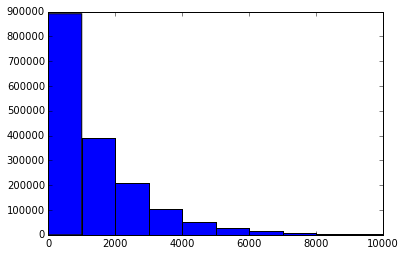
\includegraphics[width=\textwidth]{assets/01-hist.png}\strut
\end{minipage}\tabularnewline
\bottomrule
\end{longtable}

\begin{longtable}[]{@{}ll@{}}
\caption{\href{http://matplotlib.org/api/pyplot_api.html\#matplotlib.pyplot.hist2d}{\texttt{pyplot.hist2d(data1,\ data2,\ n,\ {[}{[}x1,\ x2{]},\ {[}y1,\ y2{]}{]})}}}\tabularnewline
\toprule
\begin{minipage}[b]{0.47\columnwidth}\raggedright\strut
Description\strut
\end{minipage} & \begin{minipage}[b]{0.47\columnwidth}\raggedright\strut
Example\strut
\end{minipage}\tabularnewline
\midrule
\endfirsthead
\toprule
\begin{minipage}[b]{0.47\columnwidth}\raggedright\strut
Description\strut
\end{minipage} & \begin{minipage}[b]{0.47\columnwidth}\raggedright\strut
Example\strut
\end{minipage}\tabularnewline
\midrule
\endhead
\begin{minipage}[t]{0.47\columnwidth}\raggedright\strut
Plot a 2D histogram from two datasets, with \(n^2\) bins equally spaced
between \texttt{x1} and \texttt{x2} in \texttt{x} and \texttt{y1} and
\texttt{y2} in \texttt{y}\strut
\end{minipage} & \begin{minipage}[t]{0.47\columnwidth}\raggedright\strut
\texttt{\textgreater{}\ pyplot.hist2d(}

\texttt{\textasciitilde{}\textasciitilde{}\textasciitilde{}\textasciitilde{}\textasciitilde{}\textasciitilde{}data.H1\_PX,\ data.H2\_PX,}

\texttt{\textasciitilde{}\textasciitilde{}\textasciitilde{}\textasciitilde{}\textasciitilde{}\textasciitilde{}10,\ {[}{[}0,\ 2000{]},\ {[}0,\ 4000{]}{]}}

\texttt{\textasciitilde{}\textasciitilde{})}

\texttt{\textgreater{}\ pyplot.colorbar()}

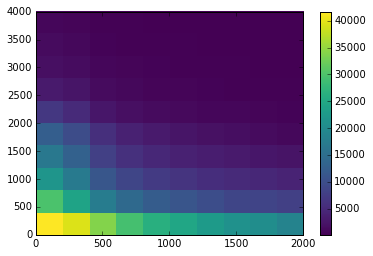
\includegraphics[width=\textwidth]{assets/02-hist2d.png}\strut
\end{minipage}\tabularnewline
\bottomrule
\end{longtable}

\begin{longtable}[]{@{}ll@{}}
\caption{\href{http://matplotlib.org/api/pyplot_api.html\#matplotlib.pyplot.scatter}{\texttt{pyplot.scatter(x,\ y,\ size,\ color)}}}\tabularnewline
\toprule
\begin{minipage}[b]{0.47\columnwidth}\raggedright\strut
Description\strut
\end{minipage} & \begin{minipage}[b]{0.47\columnwidth}\raggedright\strut
Example\strut
\end{minipage}\tabularnewline
\midrule
\endfirsthead
\toprule
\begin{minipage}[b]{0.47\columnwidth}\raggedright\strut
Description\strut
\end{minipage} & \begin{minipage}[b]{0.47\columnwidth}\raggedright\strut
Example\strut
\end{minipage}\tabularnewline
\midrule
\endhead
\begin{minipage}[t]{0.47\columnwidth}\raggedright\strut
Plot a scatter plot of \texttt{x} vs \texttt{y} where each point has
area \texttt{size} and colour \texttt{color}\strut
\end{minipage} & \begin{minipage}[t]{0.47\columnwidth}\raggedright\strut
\texttt{\textgreater{}\ pyplot.scatter(}

\texttt{\textasciitilde{}\textasciitilde{}\textasciitilde{}\textasciitilde{}\textasciitilde{}\textasciitilde{}{[}1,\ 2,\ 5,\ 1,\ 3,\ 5{]},}

\texttt{\textasciitilde{}\textasciitilde{}\textasciitilde{}\textasciitilde{}\textasciitilde{}\textasciitilde{}{[}2,\ 5,\ 1,\ 4,\ 3,\ 5{]},}

\texttt{\textasciitilde{}\textasciitilde{}\textasciitilde{}\textasciitilde{}\textasciitilde{}\textasciitilde{}40,\ "red")}

\texttt{\textasciitilde{}\textasciitilde{})}

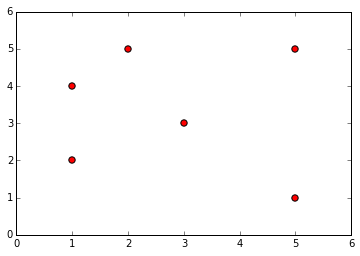
\includegraphics[width=\textwidth]{assets/03-scatter.png}\strut
\end{minipage}\tabularnewline
\bottomrule
\end{longtable}

\subsection{pandas}\label{pandas}

The following pandas functions have to be applied to an exisiting
\texttt{DataFrame} object, see the
\href{https://github.com/lhcb/opendata-project/blob/master/Example-Analysis.ipynb}{example
analysis} for a demonstration.

\begin{longtable}[]{@{}ll@{}}
\caption{\href{http://pandas.pydata.org/pandas-docs/stable/generated/pandas.DataFrame.head.html}{\texttt{df.head(n)}}}\tabularnewline
\toprule
\begin{minipage}[b]{0.47\columnwidth}\raggedright\strut
Description\strut
\end{minipage} & \begin{minipage}[b]{0.47\columnwidth}\raggedright\strut
Example\strut
\end{minipage}\tabularnewline
\midrule
\endfirsthead
\toprule
\begin{minipage}[b]{0.47\columnwidth}\raggedright\strut
Description\strut
\end{minipage} & \begin{minipage}[b]{0.47\columnwidth}\raggedright\strut
Example\strut
\end{minipage}\tabularnewline
\midrule
\endhead
\begin{minipage}[t]{0.47\columnwidth}\raggedright\strut
Produces a table of the first \texttt{n} rows of data in the
structure\strut
\end{minipage} & \begin{minipage}[t]{0.47\columnwidth}\raggedright\strut
\texttt{\textgreater{}\ df.head(3)}

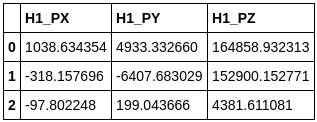
\includegraphics[width=\textwidth]{assets/04-head.png}\strut
\end{minipage}\tabularnewline
\bottomrule
\end{longtable}

\begin{longtable}[]{@{}ll@{}}
\caption{\href{http://pandas.pydata.org/pandas-docs/stable/generated/pandas.DataFrame.eval.html}{\texttt{df.eval(expression)}}}\tabularnewline
\toprule
\begin{minipage}[b]{0.47\columnwidth}\raggedright\strut
Description\strut
\end{minipage} & \begin{minipage}[b]{0.47\columnwidth}\raggedright\strut
Example\strut
\end{minipage}\tabularnewline
\midrule
\endfirsthead
\toprule
\begin{minipage}[b]{0.47\columnwidth}\raggedright\strut
Description\strut
\end{minipage} & \begin{minipage}[b]{0.47\columnwidth}\raggedright\strut
Example\strut
\end{minipage}\tabularnewline
\midrule
\endhead
\begin{minipage}[t]{0.47\columnwidth}\raggedright\strut
Evaluate an expression in the context of the DataFrame\strut
\end{minipage} & \begin{minipage}[t]{0.47\columnwidth}\raggedright\strut
\texttt{\textgreater{}\ df{[}\textquotesingle{}H1\_PT\textquotesingle{}{]}\ =\ data.eval(}

\texttt{\textasciitilde{}\textasciitilde{}\textasciitilde{}\textasciitilde{}\textasciitilde{}\textasciitilde{}\textquotesingle{}H1\_PT\ =\ sqrt(H1\_PX**2\ +\ H1\_PY**2)\textquotesingle{}}

\texttt{\textasciitilde{}\textasciitilde{})}

\texttt{df.head(3)}

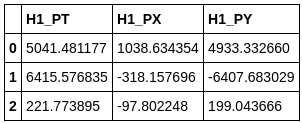
\includegraphics[width=\textwidth]{assets/05-eval.png}\strut
\end{minipage}\tabularnewline
\bottomrule
\end{longtable}

\begin{longtable}[]{@{}ll@{}}
\caption{\href{http://pandas.pydata.org/pandas-docs/stable/generated/pandas.DataFrame.min.html}{\texttt{df.min()}}}\tabularnewline
\toprule
\begin{minipage}[b]{0.47\columnwidth}\raggedright\strut
Description\strut
\end{minipage} & \begin{minipage}[b]{0.47\columnwidth}\raggedright\strut
Example\strut
\end{minipage}\tabularnewline
\midrule
\endfirsthead
\toprule
\begin{minipage}[b]{0.47\columnwidth}\raggedright\strut
Description\strut
\end{minipage} & \begin{minipage}[b]{0.47\columnwidth}\raggedright\strut
Example\strut
\end{minipage}\tabularnewline
\midrule
\endhead
\begin{minipage}[t]{0.47\columnwidth}\raggedright\strut
Return the minimum value for each column in a dataframe\strut
\end{minipage} & \begin{minipage}[t]{0.47\columnwidth}\raggedright\strut
\texttt{\textgreater{}\ df.min()}

\texttt{H1\_PX\ \ \ \ \ \ \ \ \ \ \ \ \ \ -122475.373002}

\texttt{H1\_PY\ \ \ \ \ \ \ \ \ \ \ \ \ \ -613485.901808}

\texttt{H1\_PZ\ \ \ \ \ \ \ \ \ \ \ \ \ \ \ \ \ 1420.725768}

\texttt{dtype:\ float64}\strut
\end{minipage}\tabularnewline
\bottomrule
\end{longtable}

\begin{longtable}[]{@{}ll@{}}
\caption{\href{http://pandas.pydata.org/pandas-docs/stable/generated/pandas.DataFrame.max.html}{\texttt{df.max()}}}\tabularnewline
\toprule
\begin{minipage}[b]{0.47\columnwidth}\raggedright\strut
Description\strut
\end{minipage} & \begin{minipage}[b]{0.47\columnwidth}\raggedright\strut
Example\strut
\end{minipage}\tabularnewline
\midrule
\endfirsthead
\toprule
\begin{minipage}[b]{0.47\columnwidth}\raggedright\strut
Description\strut
\end{minipage} & \begin{minipage}[b]{0.47\columnwidth}\raggedright\strut
Example\strut
\end{minipage}\tabularnewline
\midrule
\endhead
\begin{minipage}[t]{0.47\columnwidth}\raggedright\strut
Return the maximum value for each column in a dataframe\strut
\end{minipage} & \begin{minipage}[t]{0.47\columnwidth}\raggedright\strut
\texttt{\textgreater{}\ df.max()}

\texttt{H1\_PX\ \ \ \ \ \ \ \ \ \ \ \ \ \ \ 2.411849e+05}

\texttt{H1\_PY\ \ \ \ \ \ \ \ \ \ \ \ \ \ \ 1.748288e+05}

\texttt{H1\_PZ\ \ \ \ \ \ \ \ \ \ \ \ \ \ \ 1.998913e+07}

\texttt{dtype:\ float64}\strut
\end{minipage}\tabularnewline
\bottomrule
\end{longtable}

\begin{longtable}[]{@{}ll@{}}
\caption{\href{http://pandas.pydata.org/pandas-docs/stable/generated/pandas.DataFrame.query.html}{\texttt{df.query(expression)}}}\tabularnewline
\toprule
\begin{minipage}[b]{0.47\columnwidth}\raggedright\strut
Description\strut
\end{minipage} & \begin{minipage}[b]{0.47\columnwidth}\raggedright\strut
Example\strut
\end{minipage}\tabularnewline
\midrule
\endfirsthead
\toprule
\begin{minipage}[b]{0.47\columnwidth}\raggedright\strut
Description\strut
\end{minipage} & \begin{minipage}[b]{0.47\columnwidth}\raggedright\strut
Example\strut
\end{minipage}\tabularnewline
\midrule
\endhead
\begin{minipage}[t]{0.47\columnwidth}\raggedright\strut
Select part of a DataFrame provided \texttt{expression} evaluates to
true\strut
\end{minipage} & \begin{minipage}[t]{0.47\columnwidth}\raggedright\strut
\texttt{\textgreater{}\ df\_2\ =\ df.query("H1\_PX\ \textgreater{}\ 0")}

\texttt{df\_2.head(3)}

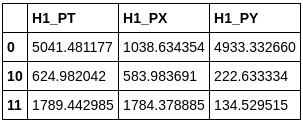
\includegraphics[width=\textwidth]{assets/06-query.png}\strut
\end{minipage}\tabularnewline
\bottomrule
\end{longtable}

\end{document}
